\documentclass[a4paper,12pt]{article}
\usepackage[utf8]{inputenc}
\usepackage{graphicx}
\usepackage{wrapfig}
\usepackage[top=1.5cm, bottom=1.5cm, left=1cm, right=1cm]{geometry}

\begin{document}
\thispagestyle{empty}

\begin{center}
    \hspace*{-2.5cm}\Huge\textbf{Ultimaker User Guide}\\
    \hspace*{-7.cm}\Large\textit{Institute of Making}
\end{center}



\vspace*{0.5cm}

\begin{wrapfigure}[8]{r}{5.5cm}
\begin{center}
{\vspace*{-1.5cm} 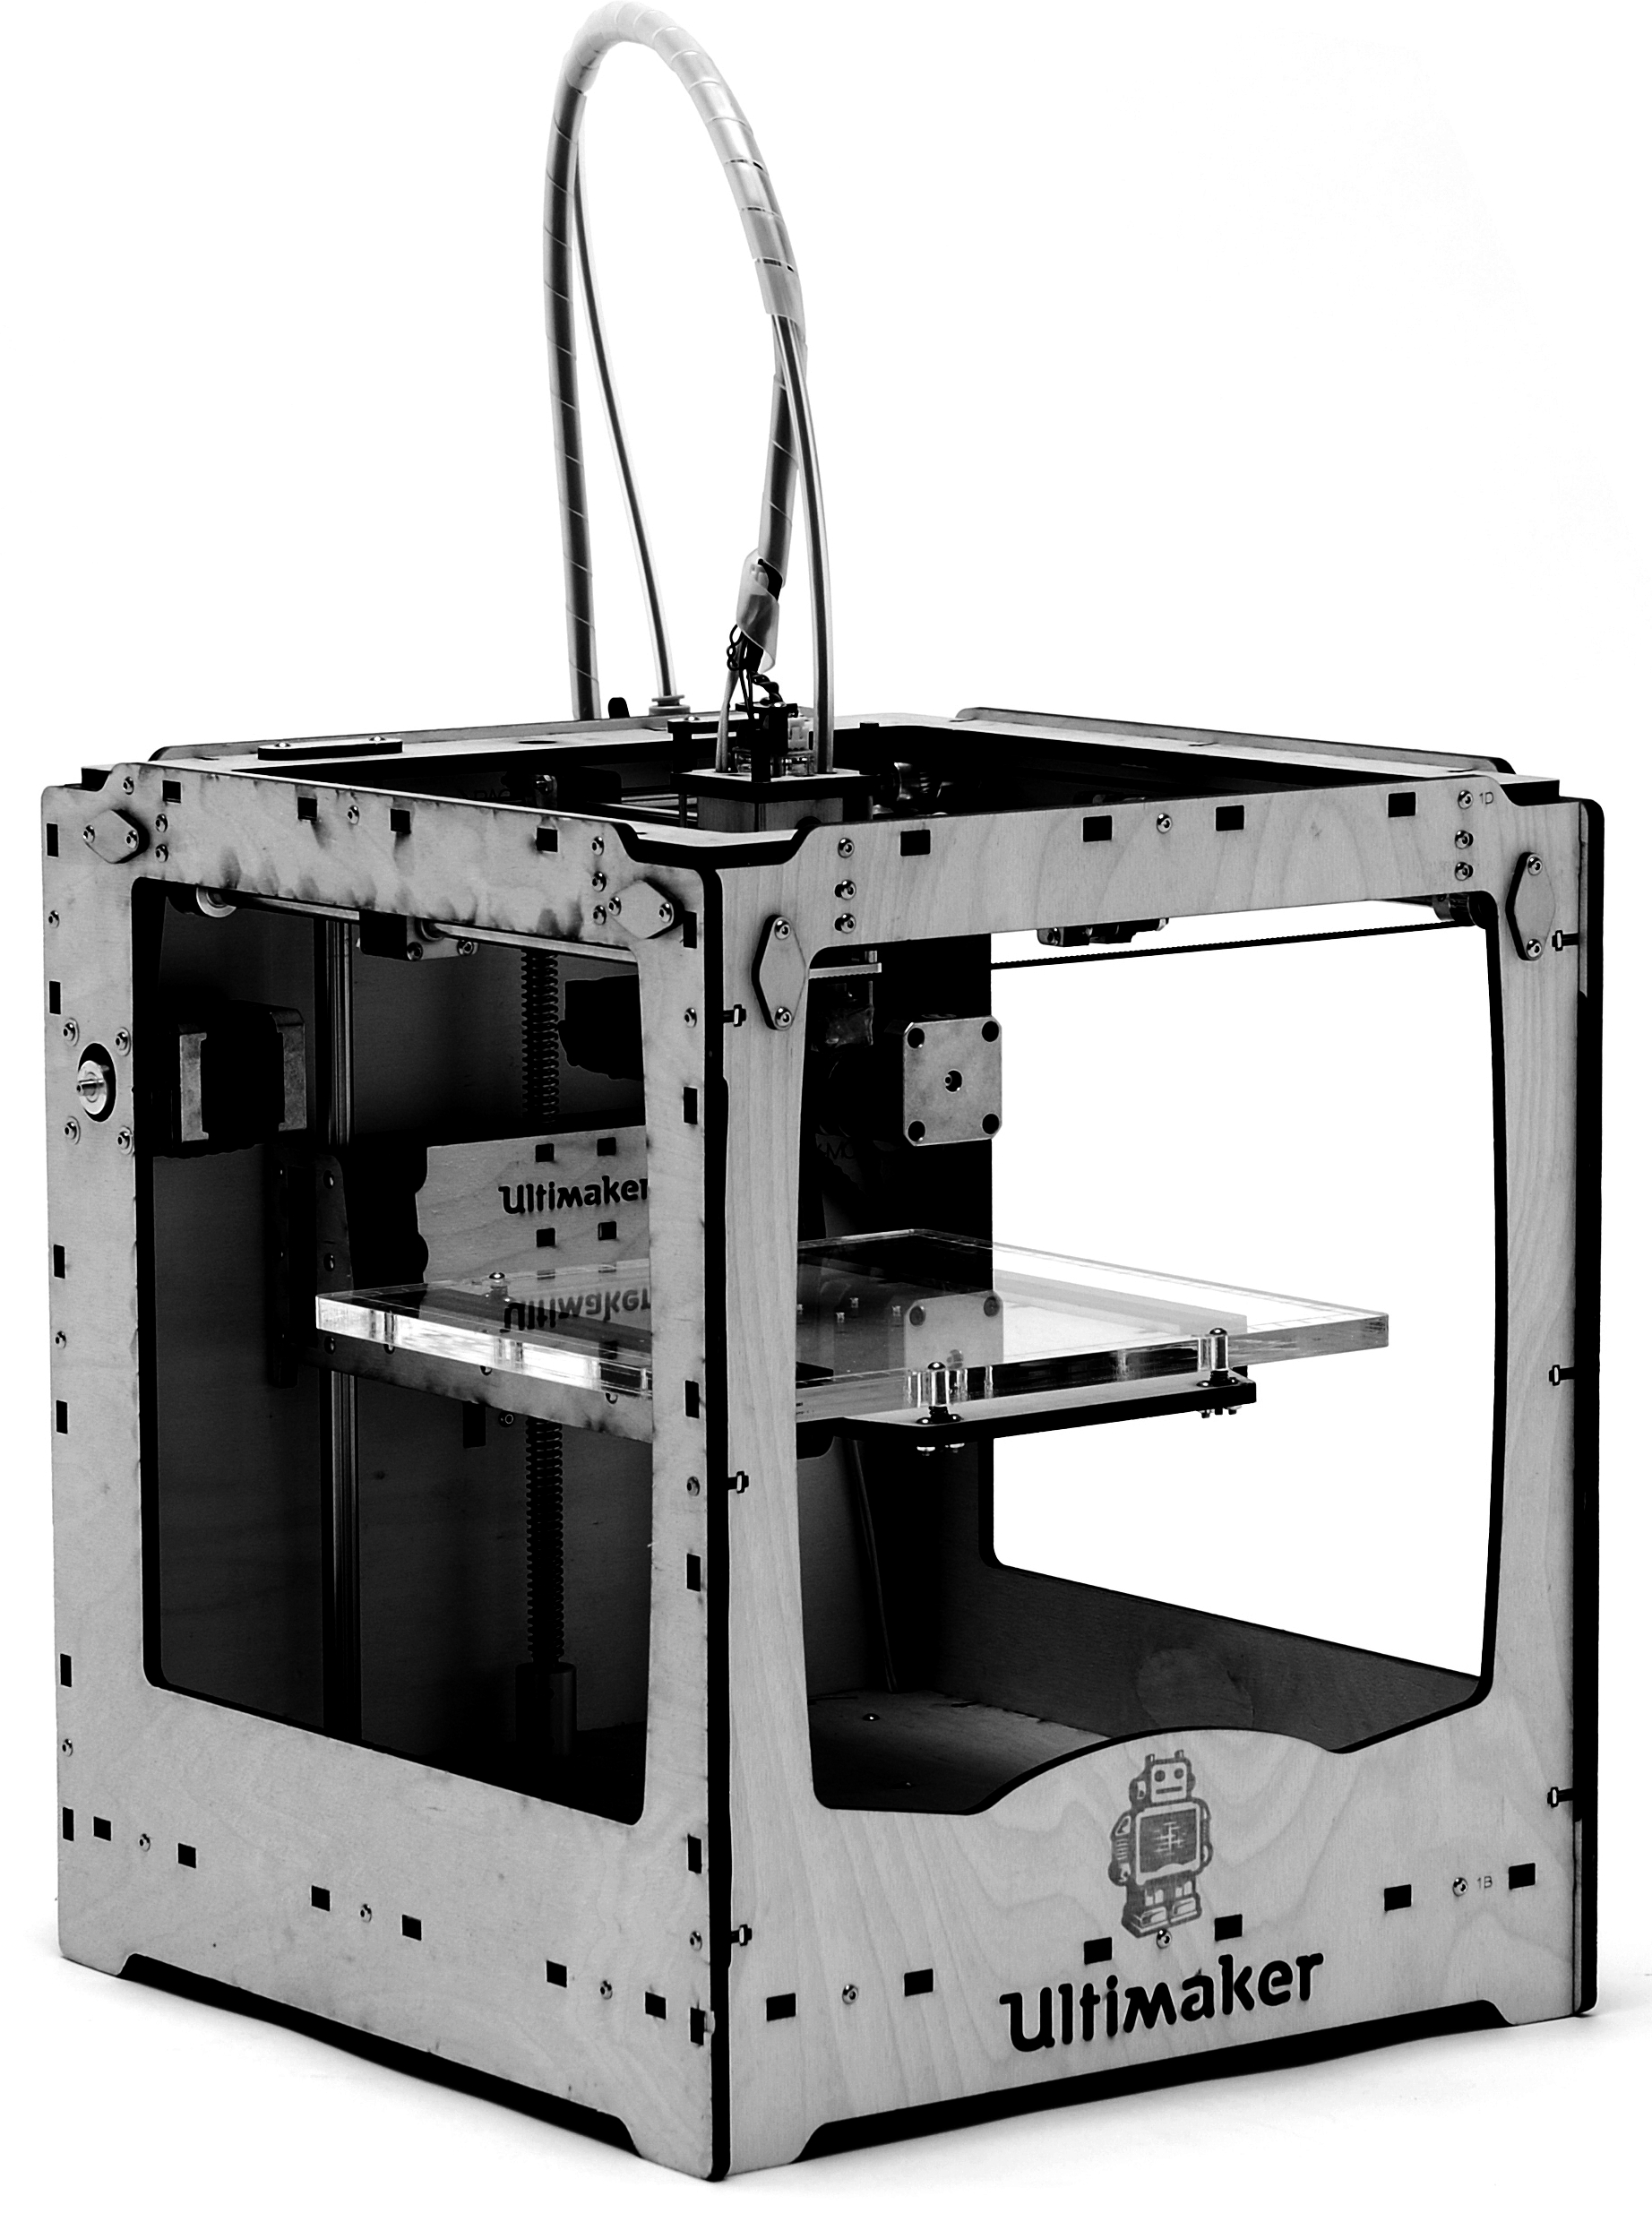
\includegraphics[width=4.5cm]{ultimaker}}
\end{center}
\end{wrapfigure}

\noindent The Ultimaker is a great machine that is capable of fast, accurate prints. It is best suited to printing PLA because it does not have a heated bed. If you want a part that is strong(er), needs finishing, or has to
survive temperatures above $50 \,^{\circ}$C, you may be better printing on one of the MakerBot 2Xs in ABS. However, this machine will produce stiff, dimensionally accurate 
parts in PLA that will not warp while printing. Because it prints in PLA it should also be better at bridging and overhangs (all of this applies to the MakerBot 2 as well).

\section*{Basic Printing}

\begin{itemize}
  \item On the Ultimaker menu select \textbf{Main $\rightarrow$ Prepare $\rightarrow$ Preheat PLA}.
  \item Load your .stl file into \textbf{Cura} on the computer.
  \item Set up print temperature, infill percentage, speed etc. as you wish and insert an SD card. If you are unsure what
  settings would be best for your print ask someone or do some small experiments. Defaults will be fine for most.
  \item Save the generated GCode onto the SD card using \textbf{File $\rightarrow$ Save GCode}. There is no `slice' button - the object is resliced (quickly!) as you adjust each setting.
  \item Eject the SD card from the computer and place it into the Ultimaker control panel.
  \item Select your print from the Ultimaker menu using \textbf{Main $\rightarrow$ Card Menu $\rightarrow$ \textit{your\_file\_here}}.
  
\end{itemize}

\section*{Tuning}
The Ultimaker is very `tweakable.' Some tweaks are semi-permanent, so unless you know what you are doing it is best to avoid anything in
the \textbf{Main $\rightarrow$ Motion} part of the menu.


However, after starting a print it is possible to tune the machine in several ways. Firstly, you can adjust the speed of the whole machine by turning the control knob left and right on the status screen. 

Secondly, after starting a print the \textbf{Main $\rightarrow$ Prepare} menu option will change to \textbf{Main $\rightarrow$ Tune}. Within this submenu you are given the options `speed' (same as above), `flow', `nozzle' and `fan speed'.

\vspace*{2mm}
\small{
\noindent \textbf{Speed} - This option affects the speed of the whole printer. It can be helpful to lower this for the first layer if your print is having problems adhering to the bed. This is 
especially likely if your first layer contains small angles. This number is a percentage, so if you sliced with a print speed of 40mm/s but change this to 150, the machine will print at 40 x 1.5 = 60mm/s.
Slower is easier for the printer.

\vspace*{2mm}
\noindent \textbf{Flow} - This affects the flowrate of the printer. If it seems that too much/too little filament is being extruded you can adjust this. 
You should not need to change this if the filament diameter is set up correctly during slicing.

\vspace*{2mm}
\noindent \textbf{Nozzle} - This is the temperature of the hot end. If your print seems `droopy' you could try lowering it. A higher temperature 
also makes it easier for the first layer to adhere. Please do not go lower than $180\,^{\circ}$C or higher than $250\,^{\circ}$C ($230\,^{\circ}$C is a sensible value).

\vspace*{2mm}
\noindent \textbf{Fan Speed} - `Droopiness' can also be cured by increasing the fan speed. This is especially useful for small details, overhangs and bridges. Cura
should take care of this during slicing but you have the option to tweak it if you want to - values go between 0 and 255.
}

\newpage
\thispagestyle{empty}
\footnotesize{

\section*{Maintenance}
Inevitably, if you use any FDM 3D printer you will enounter blocked nozzles, uneven beds, random failures and other inexplicable problems.
Rejoice in these, and be happy that you are bonding with your printer.

\vspace*{2mm}
\noindent \textbf{Replacing the Bed Lining} - If the tape covering the print bed is torn or overly greasy, your first layer will not stick and your print will fail. Replacing the tape is 
easily done. Most importantly, take some effort to make sure each strip lines up with the previous one - do not leave any gaps and do not overlap.
The layer of tape you put down needs to be even and flat.


\vspace*{2mm}
\noindent \textbf{Nozzle Unblocking} - If the printer stops extruding plastic but seems to be continuing with the print, it is likely that the nozzle is blocked. Generally at this point you will need to
stop the print, unblock the nozzle, and restart the print from scratch. After stopping the print you can move the print head around
manually via \textbf{Main $\rightarrow$ Prepare $\rightarrow$ Move Axis $\rightarrow$ 1mm $\rightarrow$ \textit{axis}}. This inlcudes retracting and extruding filament. If you only want to move the print head you can disable the 
motors (\textbf{Main $\rightarrow$ Prepare $\rightarrow$ Disable steppers}) and move it by hand. Most blockages
can be solved by retracting a few mm of filament and then re-attempting to extrude.

\vspace*{2mm}
\noindent \textbf{Bed Levelling} - Look carefully at the first layer of your print. If the line of plastic being layed down seems wider in some places than others, or seems altogether too `squashed out' or too thin,
then it is likely you need to adjust the level of the print bed. This can be done by moving the nozzle around the bed (\textbf{Main $\rightarrow$ Prepare $\rightarrow$ Move Axis $\rightarrow$ 1mm $\rightarrow$ \textit{axis}})
and adjusting the screws until you can just fit a piece of copier paper between the nozzle and the bed at any point. The most efficient way to do this is to start by homing the printer (\textbf{Main $\rightarrow$ Prepare $\rightarrow$ Auto Home}) and loosening the back right screw. Now place the nozzle next to the front left screw and adjust it until a piece of paper is lightly gripped by the nozzle. Now move the nozzle to the
front right screw and adjust, then move it to the back left screw and adjust there. Now tighten the back right screw until it makes contact with the bed.



\section*{Long-Term Calibration}
As mentioned previously, some settings affect every print. It is important to get these just right if the prints are to be 
accurate. These values are the best that have been found \textbf{so far}, but if you print something that is supposed to be 100mm wide and 
it comes out at 99mm wide, the cause is (probably) here. You can change these values on the \textbf{Main $\rightarrow$ Motion} submenu. If you do so, please
make a note here (just write on this sheet if necessary).

\vspace*{2mm}
\noindent \textbf{Scale} - These values affect the scale of every print. They are what relates the controllers concept of motor movement to physical movement of the print head
or the extruder gear.

\begin{center}
\begin{tabular}{ l c r }
  X Steps/mm & 2 \\
  Y Steps/mm & 5 \\
  Z Steps/mm & 8 \\
  E Steps/mm & 8 \\
\end{tabular}
\end{center}

\vspace*{2mm}
\noindent \textbf{Movement} - These values affect the movement of the print head and extruder gear. The motors in the Ultimaker can easily damage the machine, so some limits are placed on movements
by the controller within the printer. This includes limiting instantaneous changes in velocity (jerk) and applying acceleration when velocity changes above this value are required (this is why it is hard to 
accurately estimate the time required for a print).

\begin{center}
\begin{tabular}{ l c r }
  Acceleration & 2 \\
  XY Jerk & 5 \\
  VMax X & 8 \\
  VMax Y & 8 \\
  VMax Z & 8 \\
  VMax E & 8 \\
\end{tabular}
\end{center}

\vfill

\hrule
\vspace*{1mm}
\noindent You can get a copy of the code for this guide at https://github.com/tomcatling/IoM\_UltimakerDocs.git, feel free to contribute!

}
\end{document}
